% Snowflake Data Engineering — Chapter 1 | original manuscript draft
% Author: Arman Golbidi | Editorial snapshot: 21 October 2026
% Compile: xelatex -interaction=nonstopmode -halt-on-error Snowflake_Data_Engineering_Chapter_01.tex
% Trim: 178 x 254 mm; margins inside 23 mm / outside 17 mm / top-bottom 19 mm.
% Body: 10.75 pt / 13.65 pt leading = 1.27 line-height ratio; code: 8.75 pt.
\documentclass[11pt,twoside]{article}
\usepackage[paperwidth=178mm,paperheight=254mm,inner=23mm,outer=17mm,top=19mm,bottom=19mm,headheight=5mm,headsep=4mm,footskip=9mm]{geometry}
\usepackage{fontspec}
\setmainfont{LibertinusSerif-Regular.otf}[BoldFont=LibertinusSerif-Bold.otf,ItalicFont=LibertinusSerif-Italic.otf,BoldItalicFont=LibertinusSerif-BoldItalic.otf]
\setsansfont{LibertinusSans-Regular.otf}[BoldFont=LibertinusSans-Bold.otf,ItalicFont=LibertinusSans-Italic.otf]
\setmonofont{LibertinusMono-Regular.otf}[Scale=0.91]
\usepackage[english]{babel}
\usepackage{microtype}
\usepackage{setspace}
\setstretch{1.0}
\usepackage{titlesec,enumitem,tabularx,array,booktabs,needspace,fancyhdr,lastpage}
\usepackage[most]{tcolorbox}
\usepackage{tikz}
\usetikzlibrary{arrows.meta,positioning,fit,shapes.misc}
\usepackage{listings}
\usepackage{xcolor}
\usepackage{hyperref}
\hypersetup{colorlinks=true,urlcolor=steelblue,linkcolor=steelblue,pdfauthor={Arman Golbidi},pdftitle={Snowflake Data Engineering - Chapter 1: Introduction to Snowflake and Modern Data Engineering},pdfsubject={English technical book manuscript, first chapter, 178 x 254 mm}}
\definecolor{navy}{HTML}{15334A}
\definecolor{steelblue}{HTML}{17779B}
\definecolor{teal}{HTML}{12888A}
\definecolor{lightblue}{HTML}{ECF5F7}
\definecolor{papergray}{HTML}{F2F5F6}
\definecolor{inkgray}{HTML}{4A5862}
\definecolor{thinrule}{HTML}{CBD7DB}
\AtBeginDocument{\color{navy}\fontsize{10.75}{13.65}\selectfont}
\setlength{\parindent}{0pt}
\setlength{\parskip}{3.3pt plus 0.7pt minus 0.6pt}
\setlist[itemize]{leftmargin=4mm,itemsep=1pt,topsep=2pt,parsep=0pt}
\setlist[enumerate]{leftmargin=5mm,itemsep=1pt,topsep=2pt}
\titleformat{\section}{\sffamily\bfseries\color{navy}\fontsize{14}{17}\selectfont}{}{0pt}{}
\titlespacing*{\section}{0pt}{8pt}{4pt}
\titleformat{\subsection}{\sffamily\bfseries\color{steelblue}\fontsize{10.8}{13}\selectfont}{}{0pt}{}
\titlespacing*{\subsection}{0pt}{5pt}{1pt}
\newcommand{\topic}[2]{\subsection*{#1\quad #2}}
\newcommand{\repo}[2]{\par\begingroup\small\sffamily\color{inkgray}\textbf{Explore the source project:} #1\,\href{#2}{\,\textcolor{steelblue}{[GitHub]}}. \textit{External reference; not executed or licensed for reproduction as part of this chapter.}\par\endgroup}
\newtcolorbox{insight}[1][]{enhanced,breakable,colback=lightblue,colframe=thinrule,boxrule=.45pt,arc=1.3mm,left=2.8mm,right=2.8mm,top=1.8mm,bottom=1.8mm,before skip=5pt,after skip=5pt,#1}
\newtcolorbox{whitebox}[1][]{enhanced,breakable,colback=papergray,colframe=thinrule,boxrule=.35pt,arc=1mm,left=2.6mm,right=2.6mm,top=1.5mm,bottom=1.5mm,before skip=4pt,after skip=5pt,#1}
\lstdefinestyle{chaptercode}{basicstyle=\ttfamily\fontsize{8.75}{10.7}\selectfont,backgroundcolor=\color{papergray},frame=single,framerule=.35pt,rulecolor=\color{thinrule},breaklines=true,columns=fullflexible,keepspaces=true,showstringspaces=false,aboveskip=5pt,belowskip=5pt,xleftmargin=2mm,xrightmargin=1mm,framexleftmargin=2mm,framexrightmargin=1mm}
\lstset{style=chaptercode}
\pagestyle{fancy}
\fancyhf{}
\fancyhead[LE]{\sffamily\fontsize{7.6}{9}\selectfont\color{inkgray}\textsc{Snowflake Data Engineering}}
\fancyhead[RO]{\sffamily\fontsize{7.6}{9}\selectfont\color{inkgray}\textsc{01 / Modern Data Engineering}}
\fancyfoot[LE,RO]{\sffamily\bfseries\fontsize{8.2}{9}\selectfont\color{steelblue}\thepage}
\fancyfoot[LO,RE]{\sffamily\fontsize{7.6}{9}\selectfont\color{inkgray}Arman Golbidi \quad | \quad Chapter 01}
\renewcommand{\headrulewidth}{0.35pt}
\renewcommand{\footrulewidth}{0pt}
\setcounter{page}{9}
\raggedbottom
\begin{document}
% PAGE 9 — Chapter opening
{\sffamily\bfseries\color{teal}\fontsize{10}{12}\selectfont CHAPTER 01\quad /\quad FOUNDATIONS}\par\vspace{2mm}
{\sffamily\bfseries\color{navy}\fontsize{24}{27}\selectfont Introduction to Snowflake\par and Modern Data Engineering}\par
\vspace{1mm}{\color{steelblue}\rule{\linewidth}{1.5pt}}\par
\vspace{2mm}
{\sffamily\color{inkgray}\fontsize{11.5}{15}\selectfont From raw measurements to a trustworthy decision}\par\vspace{2mm}
At 08:00, an energy analyst opens a dashboard that shows electricity generation in Finland. The chart is current, its labels look convincing, and the query returned successfully. But the source has retried yesterday's data, two timestamps have been interpreted in local time rather than UTC, and a missing quarter-hour has quietly disappeared from the total. The platform did what it was asked to do; the information is still wrong.

This is why modern data engineering is not primarily the art of moving bytes. It is the discipline of turning uncertain, changing inputs into \emph{reliable data products} that people can interpret and use. Snowflake can provide a powerful environment for that work, but architecture, semantics, quality rules, and operational judgment remain the engineer's responsibility.

\begin{insight}
\textbf{The central question of this chapter}\par
How do we choose a data architecture that delivers correct, timely, maintainable answers without paying for complexity that our users do not need?
\end{insight}

\textbf{By the end of Chapter 1, you will be able to:}
\begin{itemize}
\item Explain the evolution from traditional warehouses to cloud-based data platforms.
\item Distinguish warehouses, lakes, lakehouses, and transactional stores by workload.
\item Explain the role of Snowflake's storage, compute, and cloud-services layers.
\item Compare batch, micro-batch, and streaming with measurable freshness requirements.
\item Draft the first requirements, metrics, and context diagram for the Finland Energy Analytics capstone.
\end{itemize}
\textbf{Prerequisites:} no Snowflake experience; elementary SQL is helpful. The guided lab can be completed offline without a paid cloud account. The architecture discussion draws on Snowflake documentation [1]; all version-dependent features require verification before publication.
\begin{whitebox}
\textbf{Reader's route}\quad Sections 1.1--1.3 build a historical and architectural mental model; 1.4--1.7 test engineering decisions; 1.8 introduces the capstone; 1.L turns the ideas into a reviewable specification. We will implement the platform incrementally in later chapters.
\end{whitebox}

% PAGE 10
\Needspace{6\baselineskip}
\section*{1.1\quad The evolution of modern data platforms}
\topic{1.1.1}{On-premises systems and traditional data warehouses}
Imagine a manufacturer with order data inside an enterprise resource planning database, meter readings in CSV files, and finance reports in spreadsheets. Ten years ago, a common response was to operate a dedicated analytical database: extract records overnight, clean and reshape them, and load the results into a central warehouse. Analysts queried that carefully managed copy rather than overloading the system that processed orders.

That architecture solved a real problem: an \emph{operational} system is optimized for timely, correct transactions, while analytical questions often scan many records, join histories, and compute aggregates. Separating them protects the daily business from an expensive reporting query. Dimensional models further help readers understand what a number means: ``electricity delivered'' requires a defined measure, grain, unit, time basis, and source.

Traditional warehouses were not a mistake. They were designed around understandable constraints: hardware procurement, fixed storage capacity, scheduled maintenance, limited processor headroom, and teams that had to decide in advance how much infrastructure to buy. Their weaknesses appeared when workload shapes changed faster than procurement cycles. A monthly reporting peak might require hardware that remained idle for the rest of the month.

\begin{whitebox}
\textbf{The architectural distinction is not old versus new.} It is \emph{which responsibilities the system centralizes}. Even on cloud infrastructure, a poorly designed pipeline can reproduce every problem of its on-premises predecessor: stale extracts, undocumented transformations, and no recovery plan.
\end{whitebox}

\begin{center}
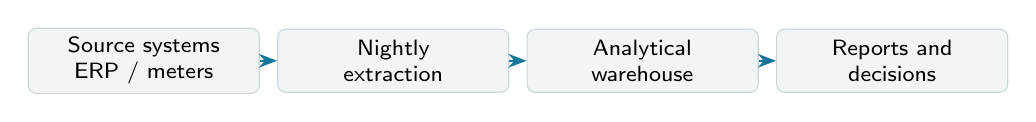
\begin{tikzpicture}[node distance=2.2mm, every node/.style={font=\sffamily\fontsize{8.3}{9.3}\selectfont}, box/.style={draw=thinrule,rounded corners=1mm,fill=papergray,minimum height=8mm,align=center,text width=27mm}, >=Stealth]
\node[box] (source) {Source systems\\ ERP / meters};
\node[box,right=of source] (batch) {Nightly\\ extraction};
\node[box,right=of batch] (dw) {Analytical\\ warehouse};
\node[box,right=of dw] (bi) {Reports and\\ decisions};
\draw[->,thick,steelblue] (source)--(batch);\draw[->,thick,steelblue] (batch)--(dw);\draw[->,thick,steelblue] (dw)--(bi);
\end{tikzpicture}
\end{center}
{\small\color{inkgray}\textbf{Figure 1.1.} A familiar scheduled warehouse pattern. The issue is not nightly loading itself, but whether its delay and failure behavior meet the reporting contract.}\par

Three questions turn the historical model into engineering judgment: \emph{How fresh must the result be?} \emph{Can the operational workload safely serve analysis?} \emph{What happens if the extract runs twice or fails halfway through?} Those questions matter regardless of the vendor.
\repo{P001: Modern Data Engineering with Snowflake}{https://github.com/Snowflake-Labs/modern-data-engineering-snowflake}

% PAGE 11
\section*{1.1\quad From fixed capacity to elastic analytics}
\topic{1.1.2}{Elastic cloud analytics and separated workloads}
Cloud platforms changed the procurement problem. Rather than purchase a machine sized for the year's busiest afternoon, a team can provision compute for a job and release it after the work ends. Snowflake applies this model through \emph{virtual warehouses}: compute clusters can be assigned to different analytical activities while accessing a common data platform. Snowflake documents three architectural layers---database storage, compute, and cloud services---which we examine in detail in Chapter 2 [1].

The separation matters because analytical workloads compete differently. A data transformation job may scan and update large tables; a dashboard may issue many smaller queries during working hours; an experimental Python notebook may be unpredictable. Assigning distinct virtual warehouses can reduce contention between these compute workloads. It does not eliminate every shared dependency, and it does not make credits free: warehouses consume credits while running, subject to billing rules and minimums [2].

\topic{1.1.3}{Evolving responsibilities of the data engineer}
Infrastructure automation also shifts work rather than removing it. Modern data engineers must design data contracts, select ingestion modes, reason about schema changes, organize testing, secure access, monitor freshness, and explain costs. They ask whether a reported number can be traced back to its source and whether a corrected upstream record will update a downstream metric safely.

\begin{insight}
\textbf{Worked decision: two teams, one dataset}\par
The energy-analysis team refreshes a daily report once each morning; an operations team investigates current power measurements throughout the day. Both can use a shared governed dataset, but the same refresh target and compute schedule need not fit both. The engineering decision is to separate \emph{service objectives} before selecting services or warehouse sizes.
\end{insight}

In Snowflake, ``elastic'' is an engineering affordance, not a performance guarantee. Starting more compute might reduce queueing, but it will not repair an incorrect join or a duplicated source file. Likewise, a high-throughput platform will not resolve the meaning of an energy statistic. Correctness begins with agreement on identifiers, units, boundaries, and acceptable delays.

\textbf{Decision checkpoint.} Suppose reporting needs only yesterday's validated totals. A scheduled batch is a defensible default. If a control room requires updates within a short interval, revisit that design with an explicit freshness target and failure budget. You should justify the extra moving parts in operational terms, not because ``streaming'' sounds more modern.

\textbf{Common failure.} Teams often equate successful pipeline execution with accurate data. A green job status proves a process completed according to its controls; it does not prove the business meaning of the result. We will add independent invariants and reconciliation checks later.

% PAGE 12
\section*{1.2\quad Data warehouses, lakes, lakehouses, and data clouds}
\topic{1.2.1}{Data warehouses and data lakes}
A \emph{data warehouse} organizes information for repeatable analytical queries. Curated tables, stable dimensions, explicit metric definitions, and well-understood access patterns make it appropriate for business intelligence. A \emph{data lake} is typically an object-storage-based collection of data in diverse formats and stages of refinement; it can accommodate raw files cheaply, but a folder of files is not by itself a governed, reliable analytics system.

The distinction is functional, not a claim that warehouses can store only tables or that lakes cannot support analytics. Snowflake accepts structured and semi-structured data, while modern engines can query files in external storage. The critical question is who manages transaction semantics, metadata, security, transformation, and performance.

\topic{1.2.2}{Lakehouse and data-cloud concepts}
A \emph{lakehouse} aims to combine open or lake-style storage with table metadata, reliable reads, and analytical processing. Apache Iceberg is one table format used in this ecosystem. Snowflake documents both Snowflake-managed storage and external-volume arrangements for Iceberg tables; those choices have different governance and operational implications [1, 3]. ``Data cloud'' is broader platform language describing governed access, processing, and collaboration around data; it is not a precise replacement for a physical architecture diagram.

\topic{1.2.3}{Selecting architecture by workload rather than marketing labels}
\begin{center}\small
\begin{tabularx}{\linewidth}{@{}p{26mm}X X@{}}\toprule
\textbf{Approach} & \textbf{Useful when} & \textbf{Question to test}\\\midrule
Warehouse & Curated BI, governed SQL metrics & Are model and query contracts stable?\\
Lake & Diverse raw files and replay history & Who enforces usable table semantics?\\
Lakehouse & Shared table formats and multiple engines & How are catalogs and writes coordinated?\\
\bottomrule\end{tabularx}
\end{center}
For our energy case, retain an auditable source snapshot and build trustworthy analytical tables. Whether the source snapshot stays in an external object store, in Snowflake-managed storage, or in both is a cost, governance, and recovery decision. It is not dictated by the word ``lakehouse.''

\textbf{Failure to avoid:} assuming an open table format means every engine supports identical semantics, security, and performance. Verify catalog behavior, write ownership, compatibility, and cross-tool tests before committing to a multi-engine architecture.
\repo{P002: Getting Started with Iceberg Tables}{https://github.com/Snowflake-Labs/sfguide-getting-started-with-iceberg-tables}

% PAGE 13
\section*{1.3\quad OLTP versus OLAP: workloads and design choices}
\topic{1.3.1}{Transactional versus analytical access patterns}
An electricity billing application may need to update one customer's payment atomically. An analyst may ask for two years of hourly electricity generation by source, region, and season. The first resembles \emph{online transaction processing} (OLTP): short operations, selective reads, concurrent updates, and carefully enforced invariants. The second resembles \emph{online analytical processing} (OLAP): scans, aggregates, joins, and historical comparisons. Both are databases; their principal workloads differ.

\topic{1.3.2}{Read/write characteristics and latency}
A workload specification should record operation mix, concurrency, data volume, read and write patterns, and acceptable latency. ``Real time'' is not a measurable target. ``An event must appear in the operational display within 60 seconds for 95\% of accepted events'' is closer, although it still needs a definition of event time and acceptance time.

Snowflake standard tables are primarily oriented toward analytics. Snowflake also documents \emph{hybrid tables}, designed for lower-latency indexed reads and writes with transactional capabilities, but their support and limitations depend on cloud region and account features [1, 4]. The existence of a transactional-oriented option does not imply that Snowflake should replace every operational database.

\topic{1.3.3}{Selecting a store for energy-meter use cases}
For the running project, imagine two independent applications. A device-registration system changes individual meter records throughout the day, while an analytical platform calculates generation trends and power-to-energy aggregates across many readings. We would ordinarily evaluate a transactional system for registration state and a governed analytical model for historical analysis, with an explicit ingestion boundary between them.

\begin{insight}
\textbf{Why granularity matters}\par
A row recording 480\,MW of average power for a 15-minute interval contributes \(480\times\tfrac{15}{60}=120\)\,MWh of energy for that interval under the stated sampling assumption. Summing MW readings alone does \emph{not} yield energy. An architecture that returns queries quickly but confuses those units is not successful.
\end{insight}

\textbf{Decision checkpoint.} Describe a requirement for a single-record correction and another for a two-year trend query. What write behavior, consistency guarantees, latency, and history will each need? Write your answers before naming a database.

\textbf{Common failure.} Running a broad reporting query directly against the transactional application during peak business hours can harm its primary duty. Isolate and govern analytical access unless a measured workload justifies otherwise.
\repo{P003: Hybrid Tables Performance Testing}{https://github.com/Snowflake-Labs/sfguide-getting-started-with-hybrid-tables-performance-testing}

% PAGE 14
\section*{1.4\quad Snowflake ecosystem and core use cases}
\topic{1.4.1}{Core platform components and SQL/Python roles}
Snowflake is a managed cloud data platform rather than software that you install on a local server. Its database storage layer manages persistent analytical data; virtual warehouses supply compute for supported SQL and Snowpark workloads; cloud services coordinate authentication, metadata, parsing, optimization, and other control functions [1]. Cloud-managed does not mean responsibility-free. The customer still defines permissions, trustworthy models, retention choices, and spending controls.

SQL is a first-class language for transformations and analysis. Python enters through connectors, Snowpark, and external tooling, among other workflows. Choosing one does not exclude the other: Python may retrieve a licensed API extract and validate it, while SQL defines the repeatable analytical model. Later chapters will distinguish where code executes and which component pays for it.

\topic{1.4.2}{Structured versus semi-structured processing}
An energy record may have a timestamp, a source category, and power measurement:\par\smallskip\centerline{\texttt{timestamp\_utc / source\_type / power\_mw}}\smallskip\noindent An API may instead return nested JSON: a time stamp, several measurements, metadata, and quality flags inside one object. Snowflake can process structured and semi-structured data [1], but accepting flexible JSON is not the same as validating its semantics. Explicit checks are needed for missing values, units, time zones, and schema drift.

\topic{1.4.3}{Business intelligence, data sharing, and AI use cases}
Three broad patterns are relevant here: prepare stable data for BI, share governed data products with authorized consumers, and apply forecasting or other models to curated features. Snowflake supports sharing selected database objects with other Snowflake accounts, using provider-controlled shares rather than naïvely exporting a separate copy in every intra-platform case [5]. Neither this feature nor AI capability eliminates privacy reviews, contract requirements, or the need to measure correctness.

\begin{whitebox}
\textbf{A small, defensible initial platform}\par
\texttt{Public energy source} \(\rightarrow\) \texttt{raw observations} \(\rightarrow\) \texttt{validated energy intervals} \(\rightarrow\) \texttt{daily metrics} \(\rightarrow\) \texttt{BI report}. Start with this traceable path. Add continuous loading, data sharing, or AI only when they serve an explicit requirement.
\end{whitebox}

\textbf{Failure to avoid.} Treating ``supported by the platform'' as ``available in every edition and region.'' Product surfaces and pricing change; use official documentation, account-specific verification, and a recorded test date.
\repo{P004: Zero to Snowflake}{https://github.com/Snowflake-Labs/sfguide-getting-started-from-zero-to-snowflake}
\repo{P005: Data Apps Demo}{https://github.com/Snowflake-Labs/sfguide-data-apps-demo}

% PAGE 15
\section*{1.5\quad The end-to-end data engineering lifecycle}
\topic{1.5.1}{Source discovery and data contracts}
A useful data product begins with people and decisions rather than tables. Who owns the source? What can a ``missing'' value mean? How often is the feed updated? Which conditions make a record acceptable? A \emph{data contract} captures such promises: schema, grain, units, identity, timeliness, provenance, and expected quality. A public API that returns JSON is only an entry point. Its schema and licensing terms must be recorded before the team builds dashboards around it.

\topic{1.5.2}{Ingestion, transformation, and validation}
The lifecycle then moves through ingestion, preservation of raw evidence, validation, transformation, and publication. Treat each boundary as a place where meaning can change. Parsing a timestamp can erase its offset. Filtering nulls can alter totals. Joining two tables at incompatible grains can multiply records. A reproducible pipeline makes such decisions inspectable.

\begin{center}

\begin{tikzpicture}[node distance=1.9mm, every node/.style={font=\sffamily\fontsize{7.7}{9}\selectfont}, box/.style={draw=thinrule,fill=lightblue,rounded corners=1mm,text width=24mm,align=center,minimum height=9mm},>=Stealth]
\node[box] (a) {Source\\ contract};\node[box,right=of a] (b) {Ingest and\\ preserve};\node[box,right=of b] (c) {Validate and\\ transform};\node[box,right=of c] (d) {Serve and\\ monitor};
\draw[->,thick,teal] (a)--(b);\draw[->,thick,teal] (b)--(c);\draw[->,thick,teal] (c)--(d);
\end{tikzpicture}
\end{center}
{\small\color{inkgray}\textbf{Figure 1.2.} Data engineering is a lifecycle of contracts, transformations, tests, and responsibility---not a one-way file copy.}\par

\topic{1.5.3}{Monitoring, quality, and maintenance}
Operational ownership begins after deployment. Useful indicators include latest source timestamp, delay to publication, rejected-record count, test failure rate, and cost by workload. A successful query is only one observation. If the source stops sending readings, yesterday's results may still look plausible; a freshness alert detects the silent failure.

\begin{insight}
\textbf{Six questions for every stage}\par
What went in? What came out? Which invariants hold? Which records were rejected? Can the step be repeated safely? Who responds when it fails? A team that can answer these questions is closer to operating a data product than a team that merely has a collection of scripts.
\end{insight}

For a daily energy report, the first useful contract might be: every accepted interval is uniquely identified by source and UTC timestamp; power is expressed in MW; energy calculations respect interval length; no dashboard is marked ``complete'' until required quality checks pass. These are proposed \emph{project requirements}, not claims about a public dataset.

\textbf{Common failure.} Monitoring only pipeline status ignores source freshness and business correctness. A row count can look normal even when all new rows are duplicates.
\repo{P006: Snowflake Northstar Data Engineering}{https://github.com/Snowflake-Labs/sfguide-snowflake-northstar-data-engineering}

% PAGE 16
\section*{1.6\quad Batch, streaming, and analytics architectures}
\topic{1.6.1}{Batch, micro-batch, and streaming models}
A batch loads a bounded set of data at scheduled or deliberate times. A micro-batch collects smaller intervals, often frequently. Streaming receives records or events continuously and typically involves state, delivery, ordering, and recovery concerns. These describe different processing patterns; they are not interchangeable promises about end-to-end latency.

Snowflake supports bulk file loading with \texttt{COPY INTO}, file-oriented continuous loading with Snowpipe, and row-oriented ingestion using Snowpipe Streaming. Their sources, compute models, latency characteristics, and costs differ [6]. A data engineer selects an ingestion pattern only after agreeing on the event-to-reporting requirement.

\topic{1.6.2}{Freshness and end-to-end latency metrics}
Define \emph{freshness} as how recently published data reflects the source, and \emph{latency} as the elapsed time across identified pipeline boundaries. If a sensor reports at 09:00 and the curated table becomes queryable at 09:08, the observed source-to-table delay is eight minutes. If the BI dashboard does not refresh until 09:30, the user's effective delay is thirty minutes. Measuring only ingestion hides the true result.

A proposed service-level objective (SLO) for a daily dashboard might be ``the previous UTC day's validated metrics are available by 08:00 Europe/Helsinki, on 99\% of scheduled days.'' For a near-live view, an SLO might instead target the 95th percentile of event-to-serving delay. These are \emph{illustrative targets}; source limitations and stakeholder needs must determine the real ones.

\topic{1.6.3}{Cost, complexity, and latency trade-offs}
\begin{center}\small
\begin{tabularx}{\linewidth}{@{}p{25mm}X X@{}}\toprule
\textbf{Pattern} & \textbf{Likely benefit} & \textbf{Operational burden}\\\midrule
Scheduled batch & Simple replay and reconciliation & Delayed availability between runs\\
Frequent micro-batch & More frequent publication & More scheduling and file overhead\\
Continuous rows & Lower ingestion delay potential & Delivery state, monitoring, paid service footprint\\
\bottomrule\end{tabularx}
\end{center}
\textbf{Decision checkpoint.} Would a 15-minute refresh meet the user's actual need? If yes, start there and test it before paying for a more elaborate architecture. If not, quantify what faster results change and design for backpressure, duplicates, and recovery.

\textbf{Failure to avoid.} Advertising ``five-second real time'' because a vendor documents a best-case ingestion figure. Benchmark the full path including external API, validation, transformations, BI refresh, and users' region [6].
\repo{P007: Time-Series and Streaming Guide}{https://github.com/Snowflake-Labs/sfguide-getting-started-with-time-series-using-snowflake-streaming-sis-ml-notebooks}
\repo{P008: Recommender Pipeline}{https://github.com/Snowflake-Labs/sfguide-recommender-pipeline}

% PAGE 17
\section*{1.7\quad When Snowflake is (and is not) the right choice}
\topic{1.7.1}{Strengths in BI, ELT, and governed sharing}
Snowflake is worth considering when multiple teams need governed analytical data, a SQL-centric transformation workflow, independently configurable compute, and managed infrastructure rather than self-operated database servers. It can reduce infrastructure work and support collaboration around shared analytical objects. These are capabilities, not proof of cost or speed superiority for a specific workload [1, 5].

For a team already using SQL and BI tools, an attractive design may be to ingest raw observations, transform them in Snowflake, and publish reusable metrics. Such a design still depends on good dimensional modeling, tested definitions, and clearly assigned ownership.

\topic{1.7.2}{Limitations, pricing, and vendor lock-in}
Costs require a workload model. Warehouse compute, serverless services, storage, transfers, and specialized features can be billed differently. A virtual warehouse billed while active is not equivalent to a free always-on process; storage and region choices also matter [2, 7]. Avoid publishing a fixed price per run without date, account assumptions, and measurement.

Operational dependencies matter too. Proprietary SQL features, security policies, managed orchestration, and some platform-specific AI functionality can increase migration cost. A customer may reasonably choose another platform when transactional latency, open multi-engine access, existing infrastructure, data sovereignty, or specific budget constraints dominate.

\topic{1.7.3}{Fair comparison criteria for alternatives}
Compare products using \emph{the same} data volume, source conditions, transformation semantics, concurrency, security constraints, recovery objectives, and cost window. Specify which systems handle metadata and storage, which execute computation, and who must operate each component. Never compare a fully warmed cached query with an uncached competitor's query and call the difference a platform result.

\begin{insight}
\textbf{Architecture decision record — a fair beginning}\par
\textbf{Context:} daily Finnish energy reporting with a small team. \textbf{Options:} SQL warehouse, open-table lakehouse, or managed analytics platform. \textbf{Criteria:} reliable source integration, reproducibility, governance, BI compatibility, staffing, monthly credits, and exit strategy. \textbf{Decision:} not yet final. Prototype the smallest adequate design, measure it, and record why alternatives were rejected.
\end{insight}

\textbf{Failure to avoid.} Buying capacity or complex streaming infrastructure before documenting a freshness requirement. In engineering, a simple solution that demonstrably meets a contract is often superior to an impressive architecture with unbounded maintenance obligations.
\repo{P009: Advanced Data Engineering with Snowflake}{https://github.com/Snowflake-Labs/advanced-data-engineering-snowflake}

% PAGE 18
\section*{1.8\quad Introducing the Finland Energy Analytics capstone}
\topic{1.8.1}{Stakeholders and business problem}
We will build a \emph{Finland Energy Analytics Platform}: a documented, testable data product that transforms licensed public energy observations into interpretable metrics. This is a teaching design, not an official Finnish energy statistic or a live production service. A system operator may care about timeliness; an analyst may care about comparability across years; a researcher may need provenance and reproducibility. Each needs a different kind of confidence in the same pipeline.

Before collecting data, define a narrow decision: \emph{How did the composition and amount of reported electricity generation change over a chosen period?} We must select sources according to available variables and permitted reuse, rather than assume every public API exposes the desired measurements.

\topic{1.8.2}{Energy generation/consumption indicators and time grain}
A metric catalogue prevents arithmetic from becoming disguised business logic. At minimum, specify metric name, source, unit, grain, aggregation rule, missing-value behavior, and timezone. Power (MW) is not energy (MWh); power averaged over a time interval must be multiplied by that interval's duration in hours to obtain an energy contribution. For time-series comparison, preserve original UTC timestamps and convert to local presentation time only with explicit daylight-saving handling.

\begin{center}\small
\begin{tabularx}{\linewidth}{@{}p{27mm}p{26mm}X@{}}\toprule
\textbf{Indicator} & \textbf{Unit / grain} & \textbf{Definition / caution}\\\midrule
Mean power & MW / 15-min & Average reported power for each valid interval\\
Interval energy & MWh / 15-min & Mean MW multiplied by 0.25 h, \emph{if} sample is an interval mean\\
Source freshness & Minutes / source & Publication time minus latest accepted event time\\
Completeness & Percent / day & Expected intervals received and accepted\\
\bottomrule\end{tabularx}
\end{center}
\topic{1.8.3}{Project roadmap across the book}
The first milestone is a specification, not a database. Chapters 3--6 will establish an environment and load/normalize sources; Chapters 7--10 will compare and implement transformations; Chapters 11--13 will deliver metrics, governance, and operations; Chapter 14 will explore carefully evaluated AI extensions; Chapter 15 will integrate and assess the end-to-end result.

\begin{whitebox}
\textbf{Scope boundary:} In Chapter 1 all figures and sample readings are synthetic. Real Finnish data will be selected after verifying each provider's available variables, API terms, citation requirements, and download limits. The case study does not claim live grid coverage or forecasts.
\end{whitebox}
\repo{P010: Predictive Grid Maintenance}{https://github.com/Snowflake-Labs/sfguide-ai-powered-predictive-grid-maintenance}
\repo{P011: Green-Energy IoT Engineering}{https://github.com/nbaubek/green-energy-iot-de-project}

% PAGE 19
\section*{1.L\quad Guided lab: design the first data product}
\topic{1.L.1}{Prerequisites, inputs, permissions, and cost guardrails}
\textbf{Goal:} turn the running scenario into three reviewable artifacts before creating a paid Snowflake account. Produce three files: \texttt{problem\_statement.md}, \texttt{requirements.md}, and \texttt{architecture\_context.svg}. Use the synthetic input below; no account, credential, warehouse, or live API is required.

\begin{whitebox}
\textbf{Synthetic input assumptions}\par
Each row represents \emph{mean power} in MW for one 15-minute UTC interval. Rows are uniquely identified by the pair (timestamp, source). The values are invented solely to check a dimensional and arithmetic decision; they are not Fingrid or Statistics Finland measurements.
\end{whitebox}
\begin{lstlisting}[language={},caption={Synthetic sample for the offline lab (energy\_sample.csv).}]
timestamp_utc,source,power_mw,minutes
2026-01-15T00:00:00Z,WIND,480,15
2026-01-15T00:15:00Z,WIND,500,15
2026-01-15T00:00:00Z,SOLAR,0,15
2026-01-15T00:15:00Z,SOLAR,0,15
\end{lstlisting}
\topic{1.L.2}{Step-by-step specification}
\begin{enumerate}
\item \textbf{Problem statement:} write one paragraph identifying the reader's question, decision, source categories, out-of-scope uses, and success criterion. Do not promise a live national statistic before identifying a source.
\item \textbf{Stakeholders:} specify an analyst, platform operator, and reviewer. Give each an explicit question and desired freshness.
\item \textbf{Metric catalogue:} define \texttt{interval\_energy\_mwh} as \(\texttt{power\_mw}\times\texttt{minutes}/60\), under the mean-power assumption. Define completeness on an expected-interval denominator.
\item \textbf{Data contract:} require UTC timestamps, known units, positive duration, source IDs, uniqueness, and a decision about rejected records.
\item \textbf{Architecture:} draw source \(\rightarrow\) ingest \(\rightarrow\) raw \(\rightarrow\) validated \(\rightarrow\) curated metric \(\rightarrow\) dashboard, adding trust boundaries and ownership.
\end{enumerate}
\textbf{Suggested first acceptance criteria:} the metric formula is traceable; source and grain are unambiguous; duplicate (timestamp, source) keys are rejected; no private credentials appear in deliverables; and a reviewer can reproduce the synthetic calculation offline.

\textbf{Operational guardrail:} the chapter requires zero Snowflake credits. For later labs, establish a separate learning account, a least-privilege role, warehouse auto-suspension, budget alerts, and cleanup steps before running cloud services [7]. Budgets are notifications and monitoring tools, not a guaranteed hard ceiling for every cost category.

% PAGE 20
\section*{1.L\quad Verify, review, and extend}
\topic{1.L.3}{A runnable offline check and expected result}
Save the CSV from the previous page as \texttt{energy\_sample.csv}. The following standard-library Python code checks uniqueness, positive durations, and the energy calculation. It has been designed to run without Snowflake; the included companion file is exercised separately from any cloud integration.
\begin{lstlisting}[language=Python,caption={Synthetic energy validation (chapter01\_lab.py).}]
import csv
from collections import defaultdict

energy = defaultdict(float)
seen = set()
with open("energy_sample.csv", newline="", encoding="utf-8") as f:
    for row in csv.DictReader(f):
        key = (row["timestamp_utc"], row["source"])
        assert key not in seen, f"Duplicate: {key}"
        seen.add(key)
        minutes = int(row["minutes"])
        assert minutes > 0, "Invalid interval"
        energy[row["source"]] += float(row["power_mw"]) * minutes / 60
print({k: round(v, 2) for k, v in sorted(energy.items())})
\end{lstlisting}
Expected output for the \emph{synthetic} file: \texttt{\{'SOLAR': 0.0, 'WIND': 245.0\}}. A duplicate \texttt{WIND} timestamp should fail the uniqueness assertion. The code does not check licensing, true signal validity, or whether values are interval averages; those are separate checks. Production validation should raise explicit errors rather than rely on assertions that Python can disable.
\topic{1.L.4}{Exercises and scoring rubric}
\textbf{Foundation:} explain why \(480\,\mathrm{MW}+500\,\mathrm{MW}\) is not itself \(980\,\mathrm{MWh}\). \textbf{Practitioner:} add a rejected row with duration zero and describe the failure. \textbf{Production-design question:} specify how you would replay late corrections without double counting. \textbf{Scoring:} requirements 25\%, metric semantics 25\%, test evidence 25\%, security/cost/limitations 25\%.

\begin{whitebox}
\textbf{Reviewer's acceptance checklist}\par
\begin{itemize}
\item A business decision and primary reader are stated clearly.
\item The metric catalogue distinguishes MW from MWh and names its time grain.
\item UTC timestamps, duplicate identity, missing data, and source rights are addressed.
\item Synthetic results are reproducible and plainly labelled synthetic.
\item The architecture records alternatives, a freshness objective, and a cost boundary.
\end{itemize}
\end{whitebox}

\textbf{Chapter summary.} Platform selection begins with the workload and its definition of correctness. Snowflake provides managed storage, compute, and cloud services, but the engineer must design the contracts, quality checks, operating model, and evidence that make results trustworthy. Chapter 2 follows a query through Snowflake's architecture.

{\small\sffamily\bfseries\color{steelblue}SELECTED TECHNICAL REFERENCES}\par
{\fontsize{8.3}{10}\selectfont\setstretch{1.0}
[1] Snowflake, \href{https://docs.snowflake.com/en/user-guide/intro-key-concepts}{Key Concepts and Architecture}.\par
[2] Snowflake, \href{https://docs.snowflake.com/en/user-guide/cost-understanding-overall}{Understanding Overall Cost}.\quad
[3] Snowflake, \href{https://docs.snowflake.com/en/user-guide/tables-iceberg-managing-external-volumes}{Iceberg External Volumes}.\par
[4] Snowflake, \href{https://docs.snowflake.com/en/user-guide/tables-hybrid}{Hybrid Tables}.\quad
[5] Snowflake, \href{https://docs.snowflake.com/en/user-guide/data-sharing-intro}{Secure Data Sharing}.\par
[6] Snowflake, \href{https://docs.snowflake.com/en/user-guide/data-load-snowpipe-intro}{Snowpipe and Ingestion Choices}.\par
[7] Snowflake, \href{https://docs.snowflake.com/en/user-guide/cost-controlling}{Controlling Cost}.\par
\textit{Documentation consulted 21 October 2026; recheck editions, regions, features, licenses, and pricing before publication.}\par}
\end{document}
